% =====================================================================
% GreenStep Challenge Admin -- Product Documentation
% CISC 480 Senior Capstone, Spring 2026
% =====================================================================
\documentclass[11pt,letterpaper]{article}

\usepackage[margin=1in]{geometry}
\usepackage{graphicx}
\usepackage{float}
\usepackage{hyperref}
\usepackage{xcolor}
\usepackage{titlesec}
\usepackage{longtable}
\usepackage{array}
\usepackage{booktabs}
\usepackage{enumitem}
\usepackage{caption}
\usepackage{listings}
\usepackage{tocloft}
\usepackage{lastpage}
\usepackage{fancyhdr}

% --- Hyperlink colors ---
\hypersetup{
  colorlinks=true,
  linkcolor=blue!60!black,
  urlcolor=blue!60!black,
  citecolor=blue!60!black,
  pdftitle={GreenStep Admin Console -- Product Documentation},
  pdfauthor={Team 2: Josh Dunlap, Eli Goldberger, Khue Vo, Rudy Vergara}
}

% --- Header / footer ---
\pagestyle{fancy}
\fancyhf{}
\lhead{\small GreenStep Admin Console -- Product Documentation}
\rhead{\small CISC 480, Spring 2026}
\cfoot{\thepage{} of \pageref{LastPage}}
\renewcommand{\headrulewidth}{0.4pt}

% --- Code listing style ---
\definecolor{codegray}{rgb}{0.95,0.95,0.95}
\definecolor{codeblue}{rgb}{0.1,0.3,0.6}
\lstset{
  basicstyle=\ttfamily\small,
  backgroundcolor=\color{codegray},
  frame=single,
  framesep=4pt,
  framerule=0pt,
  rulecolor=\color{codegray},
  xleftmargin=8pt,
  xrightmargin=8pt,
  breaklines=true,
  showstringspaces=false,
  keywordstyle=\color{codeblue}\bfseries,
  commentstyle=\color{green!50!black}\itshape,
  stringstyle=\color{red!70!black}
}

% --- Captions ---
\captionsetup{font=small,labelfont=bf}

% --- Title block ---
\title{
  \vspace{-1cm}
  \textbf{GreenStep Challenge Admin Console} \\[0.5em]
  \large Product Documentation
}
\author{
  Team 2 \\
  Josh Dunlap \quad Eli Goldberger \quad Khue Vo \quad Rudy Vergara \\[0.5em]
  CISC 480: Senior Capstone, Section 01 \\
  University of St.\ Thomas \\
  Community Partner: Minnesota Pollution Control Agency (MPCA)
}
\date{May 22, 2026}

\begin{document}
\maketitle
\thispagestyle{empty}

\vfill
\noindent
\textbf{Document Type:} Product Documentation \\
\textbf{Project:} GreenStep Challenge Admin Console \\
\textbf{Repository:} \url{https://github.com/CISC-480-GreenStep/sp26_team2_greenstepchallenge_admin} \\
\textbf{Live URL:} \url{https://greenstep.auriga.fyi} \\
\textbf{Version:} v0.9.0 \\
\textbf{Submission Date:} May 22, 2026
\vfill
\newpage

\tableofcontents
\newpage

% =====================================================================
\section{Product Requirement Document}
% =====================================================================

\subsection{Purpose}

The GreenStep Challenge Admin Console is the back-office tool that staff
at the Minnesota Pollution Control Agency (MPCA) use to design, launch,
and measure sustainability challenges across their workforce.
Before this tool, Kristin Mroz-Risse, the agency's Sustainability Program
Coordinator, ran each annual challenge as a sprawling network of
spreadsheets, manual emails, and ad hoc reporting. The admin console
replaces that workflow with a single web application backed by a managed
Postgres database, role-based access control, and a customizable
dashboard for monitoring engagement in real time.

\subsection{Target Users}

\begin{itemize}[noitemsep]
  \item \textbf{SuperAdmin} (Kristin and her direct delegates):
        full control over users, groups, challenges, templates, and
        deactivation. Can invite new admins.
  \item \textbf{Admin} (department-level coordinators): can create and
        manage challenges, groups, and templates; cannot create or
        deactivate top-level users.
  \item \textbf{GeneralUser} (the rest of MPCA staff): read-only inside
        the admin app; full participation happens in the sibling mobile
        application built by Team 1.
\end{itemize}

\subsection{Use Cases}

\subsubsection*{Use Case UC-1: Launch a sustainability challenge from a template}

\begin{longtable}{p{0.25\linewidth} p{0.7\linewidth}}
\toprule
\textbf{ID}         & UC-1 \\
\textbf{Name}       & Launch a sustainability challenge from a template \\
\textbf{Primary actor} & Admin \\
\textbf{Stakeholders} & MPCA staff (will participate); Kristin (program owner) \\
\textbf{Preconditions} & Admin is signed in; at least one challenge template exists; at least one group exists. \\
\textbf{Trigger}    & Admin clicks \textit{New Challenge} on the Challenges page. \\
\midrule
\textbf{Main flow} & \begin{enumerate}[noitemsep,leftmargin=*]
  \item Admin opens the Challenges page and clicks \textbf{New Challenge}.
  \item The Challenge Form renders with a template picker, field grid,
        and a live mobile preview on the right.
  \item Admin selects an existing template (e.g.\ ``Earth Month
        Challenge''). The form's name, description, category, status,
        and color palette are pre-filled. The chosen template's actions
        are staged for attachment after the challenge is created.
  \item Admin adjusts the start date, end date, and target group, then
        tweaks the four challenge colors using the inline color pickers.
        The mobile preview updates in real time.
  \item Admin clicks \textbf{Create Challenge}.
  \item The system validates required fields, INSERTs the challenge
        row, attaches the staged actions via \texttt{challenge\_actions},
        and writes an \texttt{activity\_logs} entry.
  \item The system redirects to \texttt{/challenges} where the new
        challenge appears in the list.
\end{enumerate} \\
\midrule
\textbf{Alternate flow A1} & At step 3, Admin skips the template picker
and fills the form from scratch. The remaining steps are unchanged. \\
\textbf{Alternate flow A2} & At step 5, validation fails (missing name
or date). The form highlights the offending field and submission is
blocked until corrected. \\
\textbf{Exception E1} & At step 6, Supabase rejects the INSERT because
the caller does not satisfy the \texttt{admin\_write} Row-Level
Security policy. The form surfaces ``Permission denied'' and the
challenge is not created. \\
\textbf{Postconditions} & A new row exists in \texttt{challenges};
N rows exist in \texttt{challenge\_actions}; one new row exists in
\texttt{activity\_logs}; the participantCount column starts at zero. \\
\bottomrule
\end{longtable}

\subsubsection*{Use Case UC-2: Triage engagement mid-challenge}

\begin{longtable}{p{0.25\linewidth} p{0.7\linewidth}}
\toprule
\textbf{ID}         & UC-2 \\
\textbf{Name}       & Triage engagement mid-challenge \\
\textbf{Primary actor} & Admin or SuperAdmin \\
\textbf{Stakeholders} & Kristin (program owner); challenge participants
who may need a nudge \\
\textbf{Preconditions} & At least one challenge is in \texttt{Active}
status with participants and logged actions. \\
\textbf{Trigger}    & Admin opens the dashboard during a running
challenge. \\
\midrule
\textbf{Main flow} & \begin{enumerate}[noitemsep,leftmargin=*]
  \item Admin lands on the dashboard. The default layout renders the
        Active Challenges, Top Participants, Recent Activity, and
        Participation Breakdown widgets.
  \item Admin filters the dashboard to the running challenge using the
        per-page challenge filter chip. All widgets refresh.
  \item Admin scans the Top Participants widget and notes the long
        tail of users with zero or one logged actions.
  \item Admin opens the dashboard's Customize panel and applies the
        \textit{Analytics Deep Dive} layout preset to expose the
        Participation Report widget.
  \item Admin filters the Participation Report by date range (e.g.\
        the last 7 days) and exports a CSV.
  \item Admin opens the CSV in Excel, identifies users with no
        activity, and follows up by email outside the system.
\end{enumerate} \\
\midrule
\textbf{Alternate flow A1} & At step 4, Admin instead drags an
existing widget to resize it; the new layout is persisted to
\texttt{localStorage} and survives a page refresh. \\
\textbf{Exception E1} & At step 5, if no rows match the filter, the
table renders an empty state (``No participation in this range'') and
the Export button is disabled. \\
\textbf{Postconditions} & A CSV download has been triggered; no
database state is modified; the dashboard layout for this user is
updated in \texttt{localStorage}. \\
\bottomrule
\end{longtable}

\subsection{User Stories}

The following four user stories were prioritized for the spring 2026
release. Each carries explicit acceptance criteria.

\subsubsection*{US-1 -- Passwordless sign-in}

\textit{As an MPCA staff member, I want to sign in to the admin console
using a one-time code emailed to me so that I don't have to manage yet
another password.}

\textbf{Acceptance criteria:}
\begin{itemize}[noitemsep]
  \item Entering an unregistered email shows ``Email not recognized''
        without sending a code.
  \item Entering a registered \texttt{Active} email triggers an
        8-digit code delivered via Supabase Auth within 30 seconds.
  \item Entering a registered \texttt{Deactivated} email shows
        ``Account deactivated'' and does \emph{not} send a code.
  \item Submitting the correct code within its TTL completes sign-in
        and lands the user on the dashboard.
  \item Submitting an incorrect code shows an inline error and leaves
        the form populated.
\end{itemize}

\subsubsection*{US-2 -- Create a custom group}

\textit{As an admin, I want to create a group (department, cohort, or
city) with a name and description so that I can scope a challenge to a
specific population.}

\textbf{Acceptance criteria:}
\begin{itemize}[noitemsep]
  \item Only Admin and SuperAdmin roles see the ``New Group'' button.
  \item Group name is required; description is optional.
  \item The new group appears immediately in the Groups list with
        member count = 0 and challenge count = 0.
  \item The group can be selected as the target of a new challenge
        without a page refresh.
\end{itemize}

\subsubsection*{US-3 -- Customize the dashboard}

\textit{As an admin, I want to rearrange and resize dashboard widgets
so that the metrics I check daily are visible without scrolling.}

\textbf{Acceptance criteria:}
\begin{itemize}[noitemsep]
  \item Clicking ``Customize'' enters edit mode; widgets gain a grip
        handle and resize corners.
  \item Widgets can be dragged to any 12-column grid cell and resized
        from any corner.
  \item ``Save'' persists the layout to \texttt{localStorage} for the
        current user.
  \item ``Cancel'' restores the layout that was active when edit mode
        was entered.
  \item Applying a Quick Layout Preset (Default, Executive Summary,
        Analytics Deep Dive, Compact Overview) overwrites the visible
        layout but does not save until the user clicks Save.
  \item The layout survives a hard page refresh.
\end{itemize}

\subsubsection*{US-4 -- Export a participation report}

\textit{As an admin, I want to export a filtered participation report
to CSV so that I can share it with leadership in their preferred
format.}

\textbf{Acceptance criteria:}
\begin{itemize}[noitemsep]
  \item The report can be filtered by challenge and by a date range.
  \item The export button is disabled when zero rows match the
        current filter.
  \item The exported CSV contains the visible columns: User, Challenge,
        Action, Category, Date, Notes.
  \item Filenames follow the pattern \texttt{participation-YYYY-MM-DD.csv}.
  \item User and Challenge cells in the on-screen table are clickable
        and navigate to the corresponding detail page.
\end{itemize}

\newpage

% =====================================================================
\section{User Experience and Interface Design Specification}
% =====================================================================

\subsection{User Assumptions}

\begin{itemize}[noitemsep]
  \item Users are MPCA staff with intermediate computer literacy;
        comfortable with web applications such as Outlook, SharePoint,
        and Concur.
  \item Users access the admin console primarily from a corporate
        laptop on the MPCA network; secondary access from personal
        devices is supported but not the primary use case.
  \item Users are familiar with the GreenStep program's vocabulary
        (``Action,'' ``Challenge,'' ``Category''). Onboarding new
        admins outside MPCA may require glossary support that lives
        outside this product.
  \item English is the only supported language for the initial release.
  \item Users have a corporate email account that can receive the
        OTP code in under one minute.
\end{itemize}

\subsection{Usage Constraints}

\begin{itemize}[noitemsep]
  \item \textbf{Network:} The application requires a live internet
        connection; there is no offline mode. The static SPA bundle
        is served from Vercel's global edge network and all data
        round-trips go to Supabase over HTTPS.
  \item \textbf{Browser:} Tested on the current versions of Chrome,
        Edge, Safari, and Firefox. The application targets modern
        evergreen browsers; IE 11 is explicitly not supported.
  \item \textbf{Email scanners:} MPCA staff inboxes are protected by
        corporate link-scanning that pre-fetches one-time URLs. For
        that reason the auth flow uses an 8-digit OTP code rather
        than a magic link.
  \item \textbf{Data residency:} All data lives in Supabase's
        US-East-1 region.
  \item \textbf{Mobile:} The admin app is responsive but optimized
        for desktop. Field-level data entry (e.g.\ logging a
        completed action) happens in the sibling mobile app, not
        here.
\end{itemize}

\subsection{User Story Map}

Figure~\ref{fig:storymap} shows the admin's mental model of the
product, with the backbone (left to right) tracing the typical
program cycle and stories grouped into MVP, polish, and future
releases.

\begin{figure}[H]
  \centering
  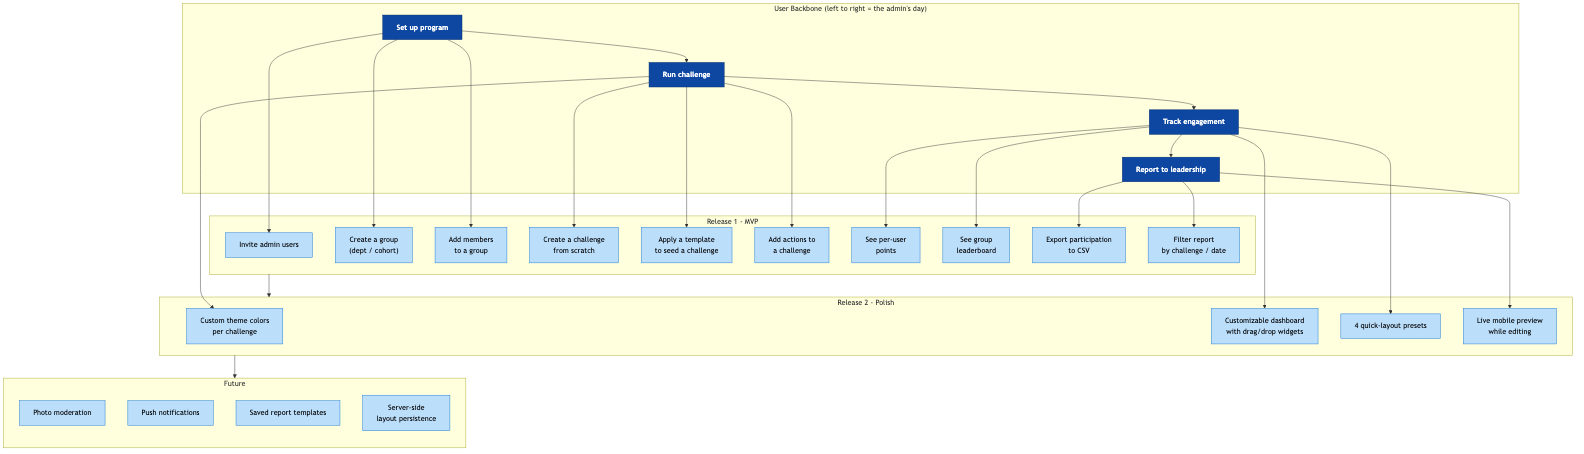
\includegraphics[width=\linewidth]{diagrams/08_user_story_map.png}
  \caption{User story map. The horizontal backbone follows the
  admin's program-management workflow; vertical slices are
  prioritized into Release 1 (MVP, shipped), Release 2 (polish,
  shipped), and Future (handed off).}
  \label{fig:storymap}
\end{figure}

\subsection{User Journey}

Figure~\ref{fig:journey} traces a representative admin journey
across the lifecycle of a single multi-week challenge, showing
where the product currently delights (mobile preview, dashboard
filtering, CSV export) and where friction remains (manual
follow-up to dormant users).

\begin{figure}[H]
  \centering
  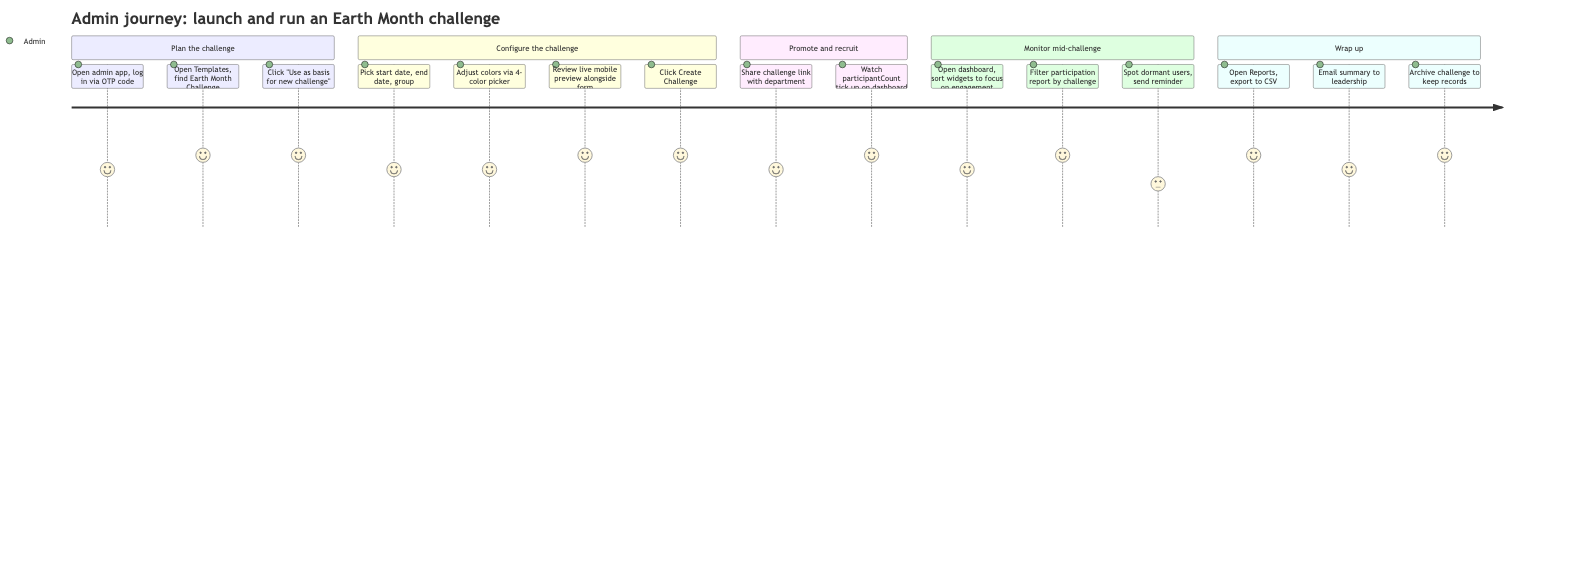
\includegraphics[width=0.95\linewidth]{diagrams/09_user_journey.png}
  \caption{Admin user journey: launching and running an Earth Month
  challenge. Higher numbers indicate higher admin satisfaction
  at that step.}
  \label{fig:journey}
\end{figure}

\subsection{Accessibility and Inclusive Design Considerations}

\begin{itemize}
  \item \textbf{Color contrast.} The MUI v7 dark theme in
        \texttt{src/lib/theme.js} was chosen partly for accessibility:
        brand greens are layered on dark surfaces with contrast
        ratios at or above WCAG AA for body text. Challenge color
        pickers default to the seeded MPCA palette, but the admin
        is free to choose any hex color, including low-contrast
        combinations -- this is a documented trade-off in favor of
        creative freedom.
  \item \textbf{Keyboard navigation.} All interactive elements are
        rendered through MUI components which carry native keyboard
        affordances (tab order, enter/space activation, focus
        rings). The dashboard's drag-and-drop grid is the one
        exception; keyboard-only users cannot currently reorder
        widgets and must rely on the Quick Layout Presets instead.
  \item \textbf{Screen readers.} Form fields are labeled (MUI
        \texttt{TextField label}) so they announce correctly. Custom
        clickable counts on list pages use \texttt{<button>} rather
        than \texttt{<div onClick>} so they are reachable via
        assistive tech.
  \item \textbf{Cognitive load.} The Customize Dashboard panel
        applies several HCI principles: affordance cues (grip
        handles, dashed borders in edit mode), feedback (snackbar
        confirmations after save), error prevention (cannot remove
        every widget; cancel/reset always available), and
        progressive disclosure (edit controls only appear once
        edit mode is engaged).
  \item \textbf{Language.} The product is English-only. The
        Action and Category vocabulary was adapted directly from
        MPCA's existing GreenStep program so the language matches
        what staff already use.
\end{itemize}

\newpage

% =====================================================================
\section{Technical Design Document}
% =====================================================================

\subsection{Architectural Overview}

The system is a single-page React 19 application hosted on Vercel
that talks directly to a managed Supabase project. Authorization
is enforced not in the React code but inside Postgres via
Row-Level Security (RLS) policies that read the role claim from
the caller's JWT. Two narrow Vercel serverless functions exist
for privileged operations that cannot be performed with the
anon key (inviting a user, hard-flipping the active status of
a user account).

\subsection{C4 -- Level 1: System Context}

Figure~\ref{fig:c4l1} shows the admin console in its environment.
The two human actors are MPCA staff (using this admin app) and
challenge participants (using the sibling mobile app built by
Team 1). Both apps share a single Supabase database.

\begin{figure}[H]
  \centering
  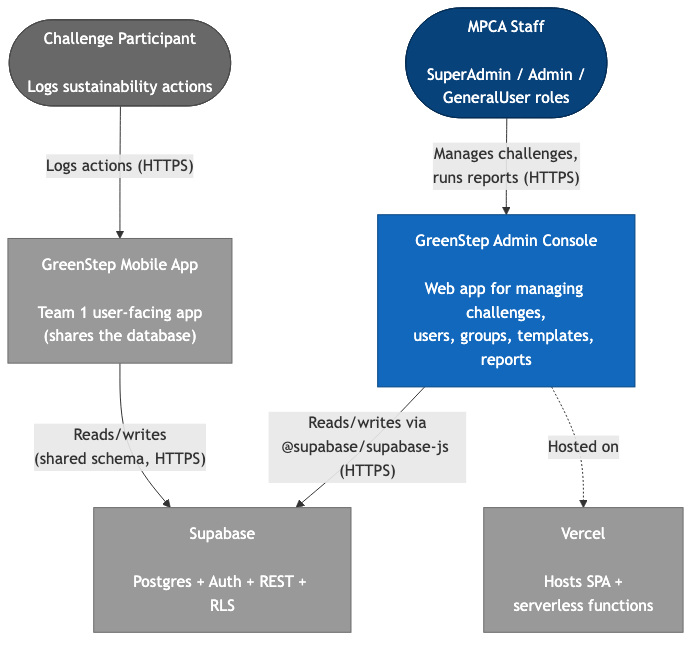
\includegraphics[width=\linewidth]{diagrams/01_c4_context.png}
  \caption{C4 Level 1 -- System context diagram.}
  \label{fig:c4l1}
\end{figure}

\subsection{C4 -- Level 2: Containers}

Figure~\ref{fig:c4l2} shows the deployable units inside the
admin console's boundary. The crucial design decision is that
the React SPA talks to Supabase directly with the anon key;
authorization lives in RLS policies, not in a middle-tier API.

\begin{figure}[H]
  \centering
  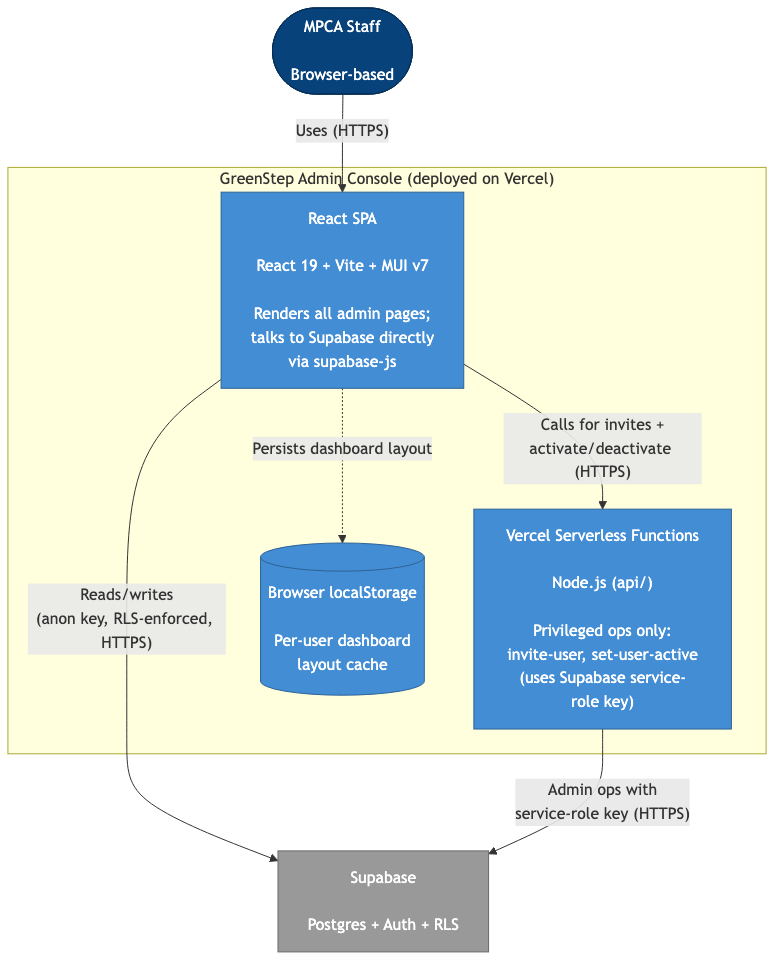
\includegraphics[width=\linewidth]{diagrams/02_c4_container.png}
  \caption{C4 Level 2 -- Container diagram. The SPA bypasses the
  need for a custom backend by relying on RLS to enforce
  authorization at the database layer.}
  \label{fig:c4l2}
\end{figure}

\subsection{C4 -- Level 3: Components inside the SPA}

Figure~\ref{fig:c4l3} shows how the SPA is organized internally,
mirroring the source tree under \texttt{src/admin-app/src/}.

\begin{figure}[H]
  \centering
  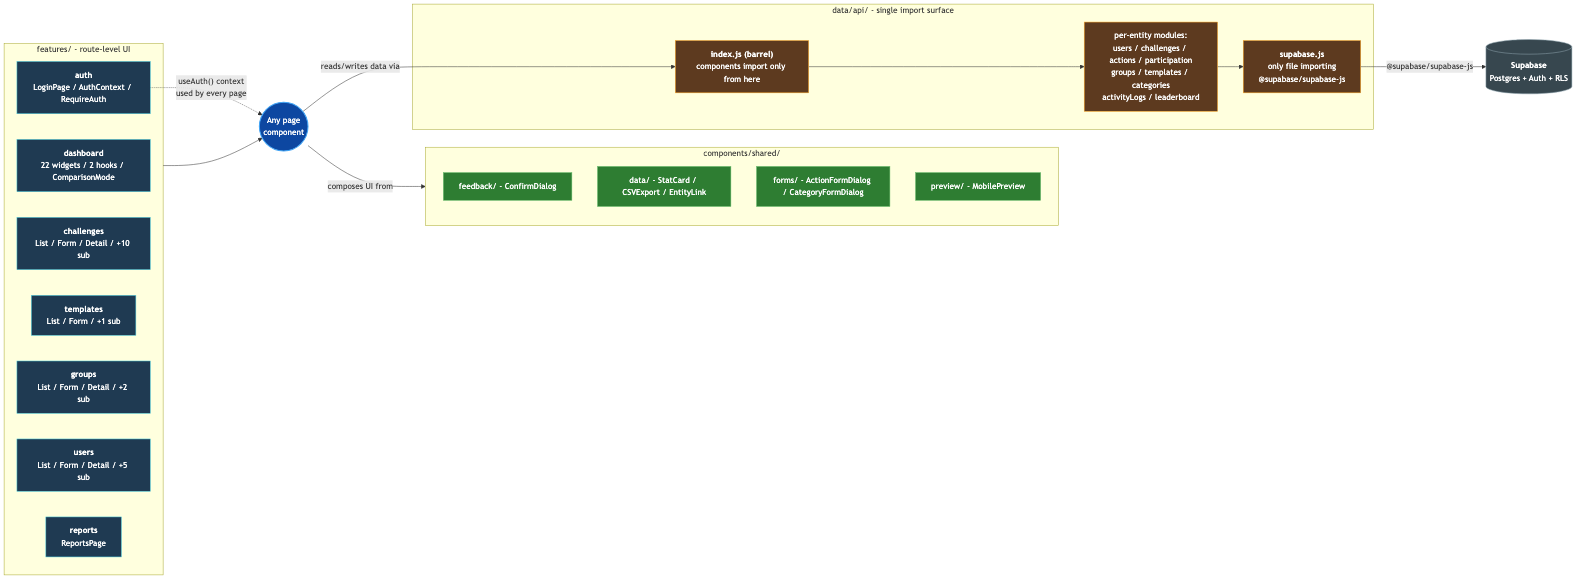
\includegraphics[width=\linewidth]{diagrams/03_c4_component.png}
  \caption{C4 Level 3 -- SPA component view. Page components
  compose UI from \texttt{components/shared} and read/write data
  through the \texttt{data/api} barrel; only one file
  (\texttt{data/supabase.js}) imports the Supabase SDK.}
  \label{fig:c4l3}
\end{figure}

\subsubsection*{Verified architectural invariants}

\begin{enumerate}[noitemsep]
  \item Only \texttt{data/supabase.js} imports
        \texttt{@supabase/supabase-js}. (Grep: 1 match.)
  \item No component bypasses the \texttt{data/api} barrel to
        import a sub-module directly. (Grep: 0 matches.)
  \item Cross-feature components live in \texttt{components/shared/}.
        No feature folder imports another feature's components.
  \item \texttt{lib/} stays small: 3 files
        (\texttt{constants.js}, \texttt{permissions.js},
        \texttt{theme.js}).
\end{enumerate}

\subsection{Data Design}

Figure~\ref{fig:er} shows the entity-relationship diagram for the
deployed Postgres schema. The schema is consolidated into the
single migration file \texttt{supabase/migrations/001\_initial\_schema.sql}.

\begin{figure}[H]
  \centering
  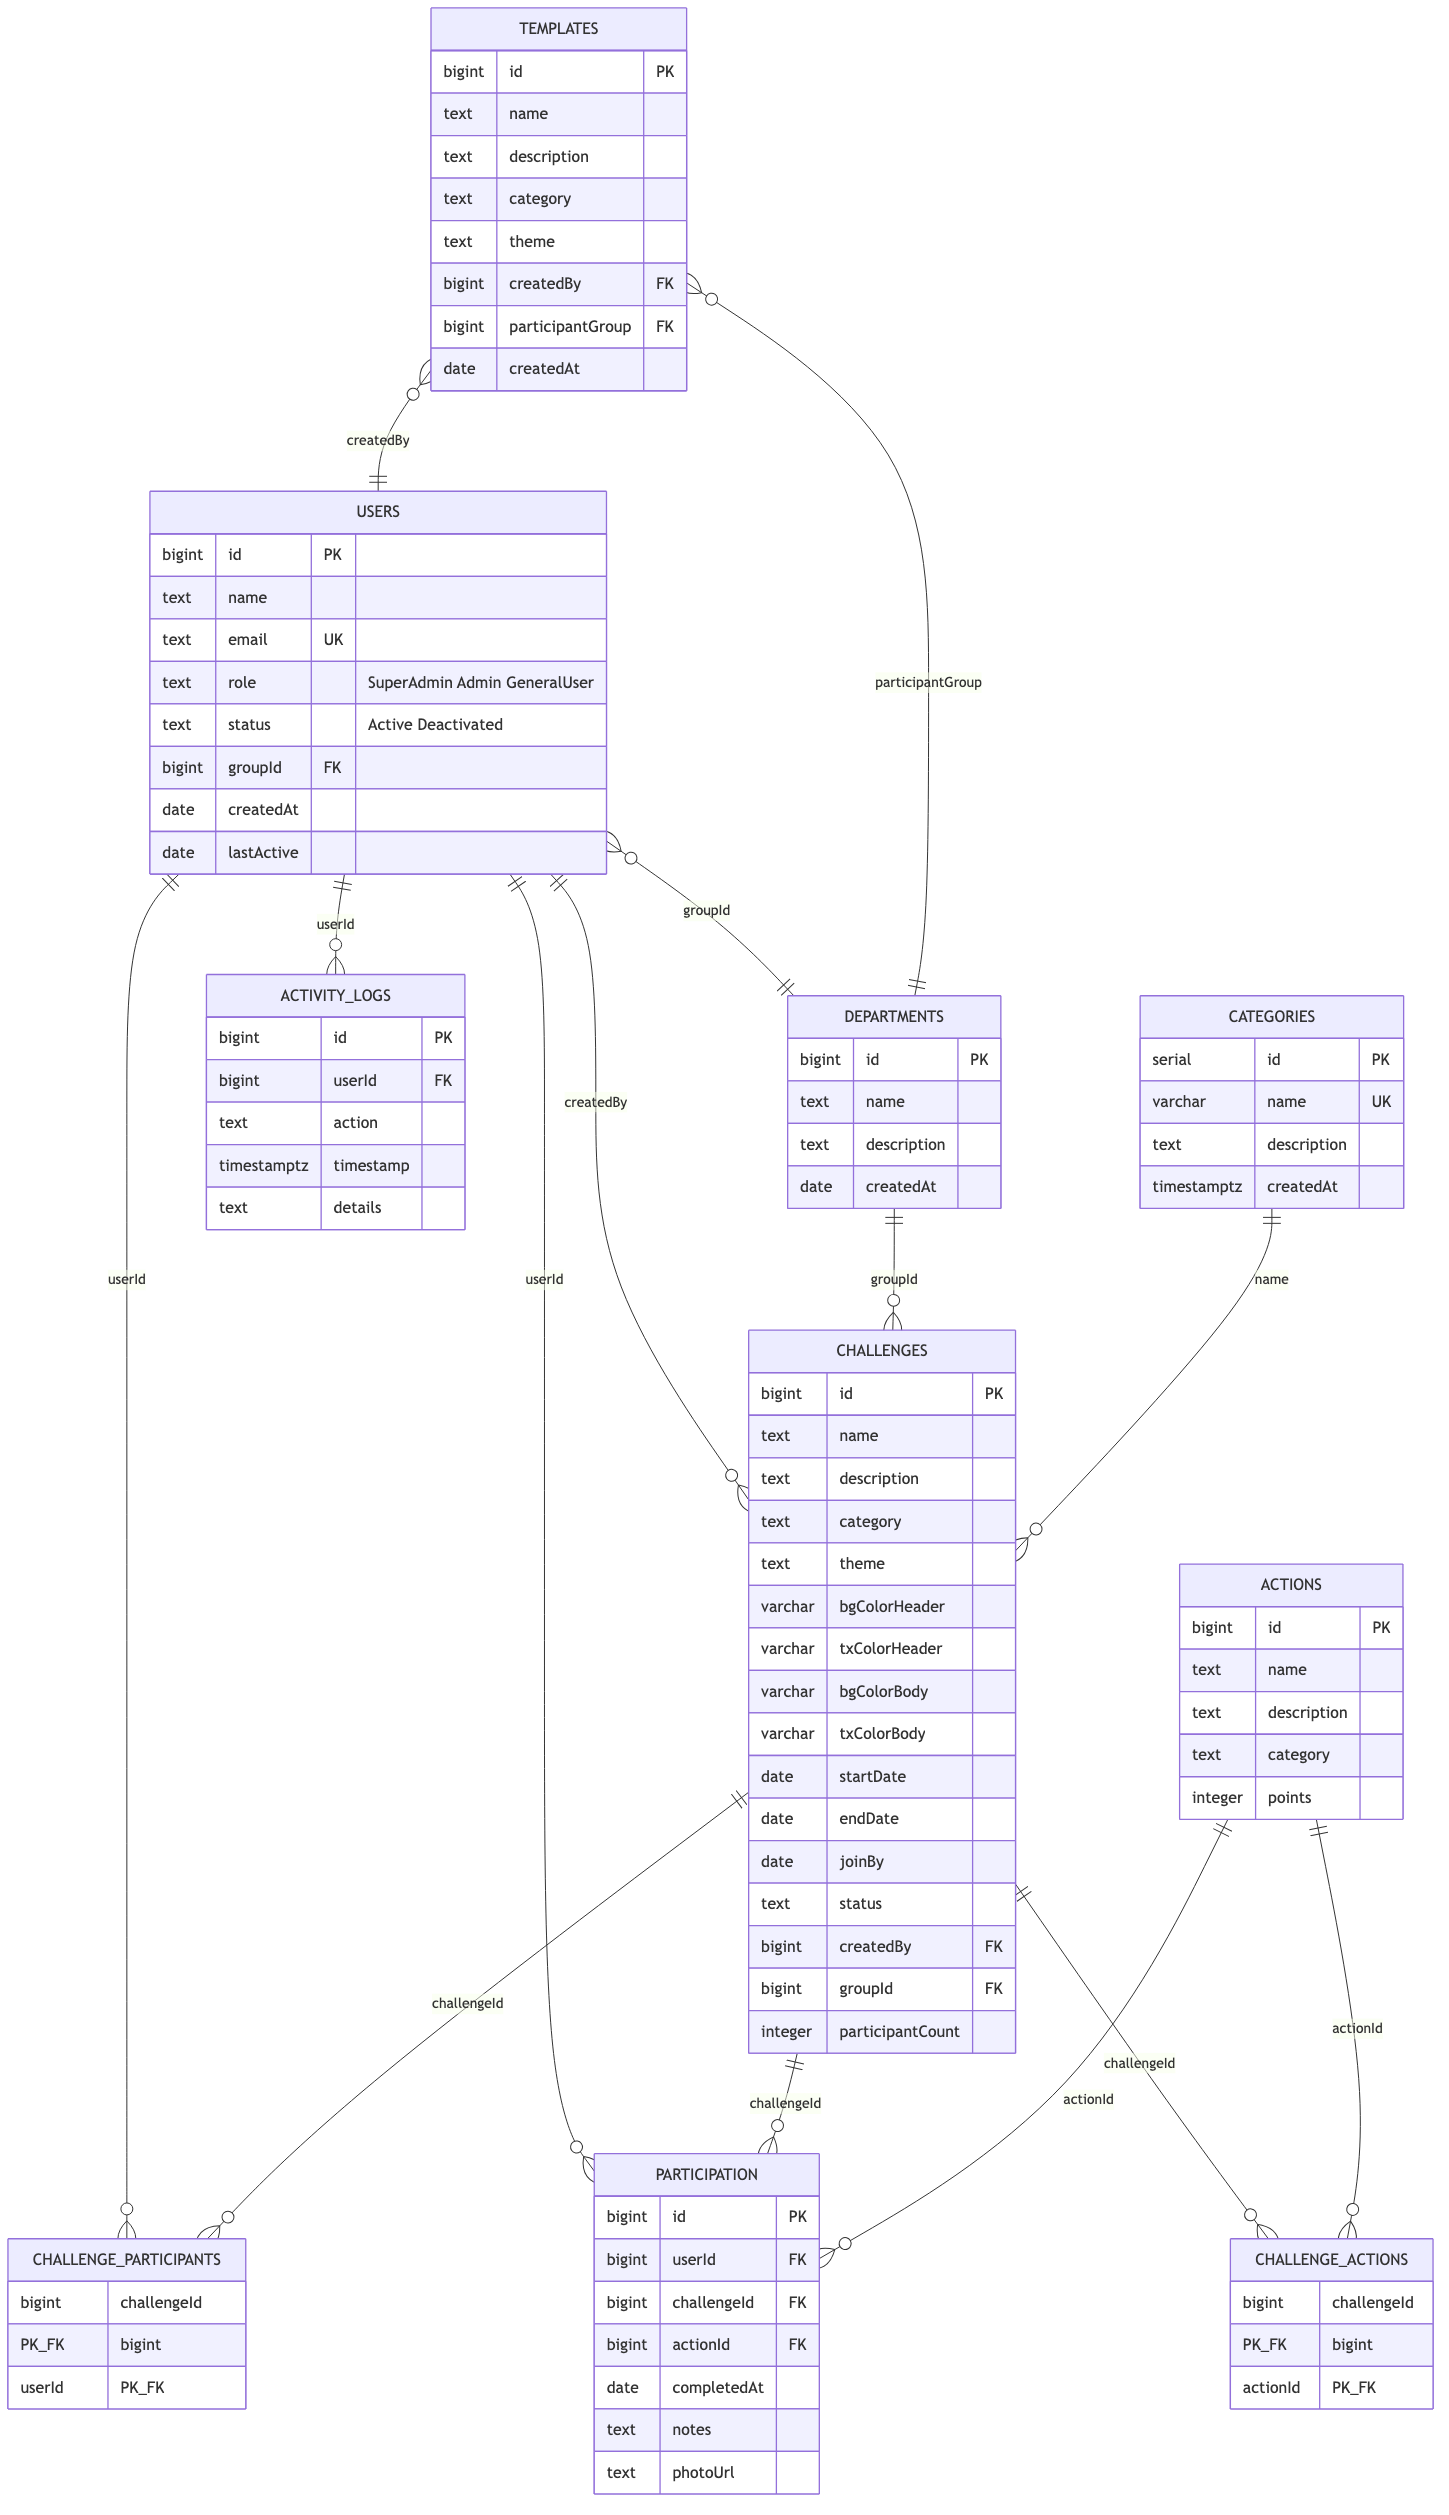
\includegraphics[width=\linewidth]{diagrams/04_er_diagram.png}
  \caption{Entity-relationship diagram for the deployed schema.
  Two many-to-many join tables (\texttt{challenge\_actions},
  \texttt{challenge\_participants}) connect challenges to their
  actions and members. The legacy single-color \texttt{theme}
  column on \texttt{challenges} coexists with the four
  \texttt{bgColor*}/\texttt{txColor*} columns added in
  migration 014.}
  \label{fig:er}
\end{figure}

\subsection{Sequence Diagram: Login (US-1)}

Figure~\ref{fig:seq-login} shows the OTP-code login flow. The
pre-flight \texttt{auth\_email\_is\_registered} RPC is a
\texttt{security definer} function that runs without RLS so
the anon-keyed client can ask ``does this email exist and is
the account active?'' without being able to read the
\texttt{users} table directly.

\begin{figure}[H]
  \centering
  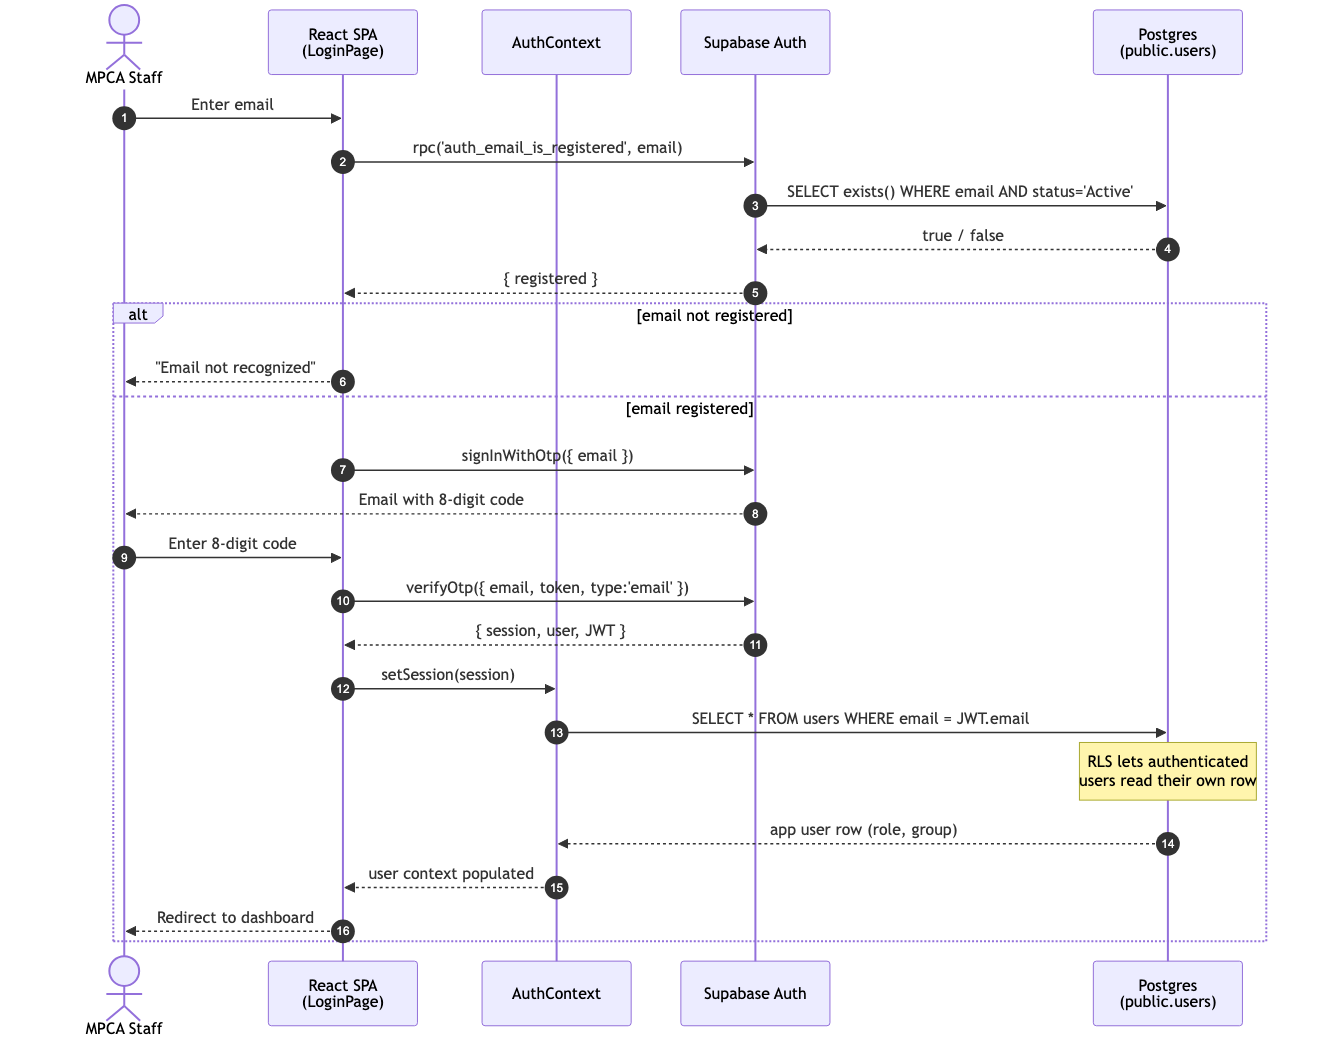
\includegraphics[width=\linewidth]{diagrams/05_seq_login.png}
  \caption{Sequence diagram -- 8-digit OTP login flow.}
  \label{fig:seq-login}
\end{figure}

\subsection{Sequence Diagram: Create Challenge (UC-1)}

Figure~\ref{fig:seq-cc} traces the create-challenge flow,
including the three parallel pre-flight reads (categories,
groups, templates) and the RLS check that gates the INSERT.

\begin{figure}[H]
  \centering
  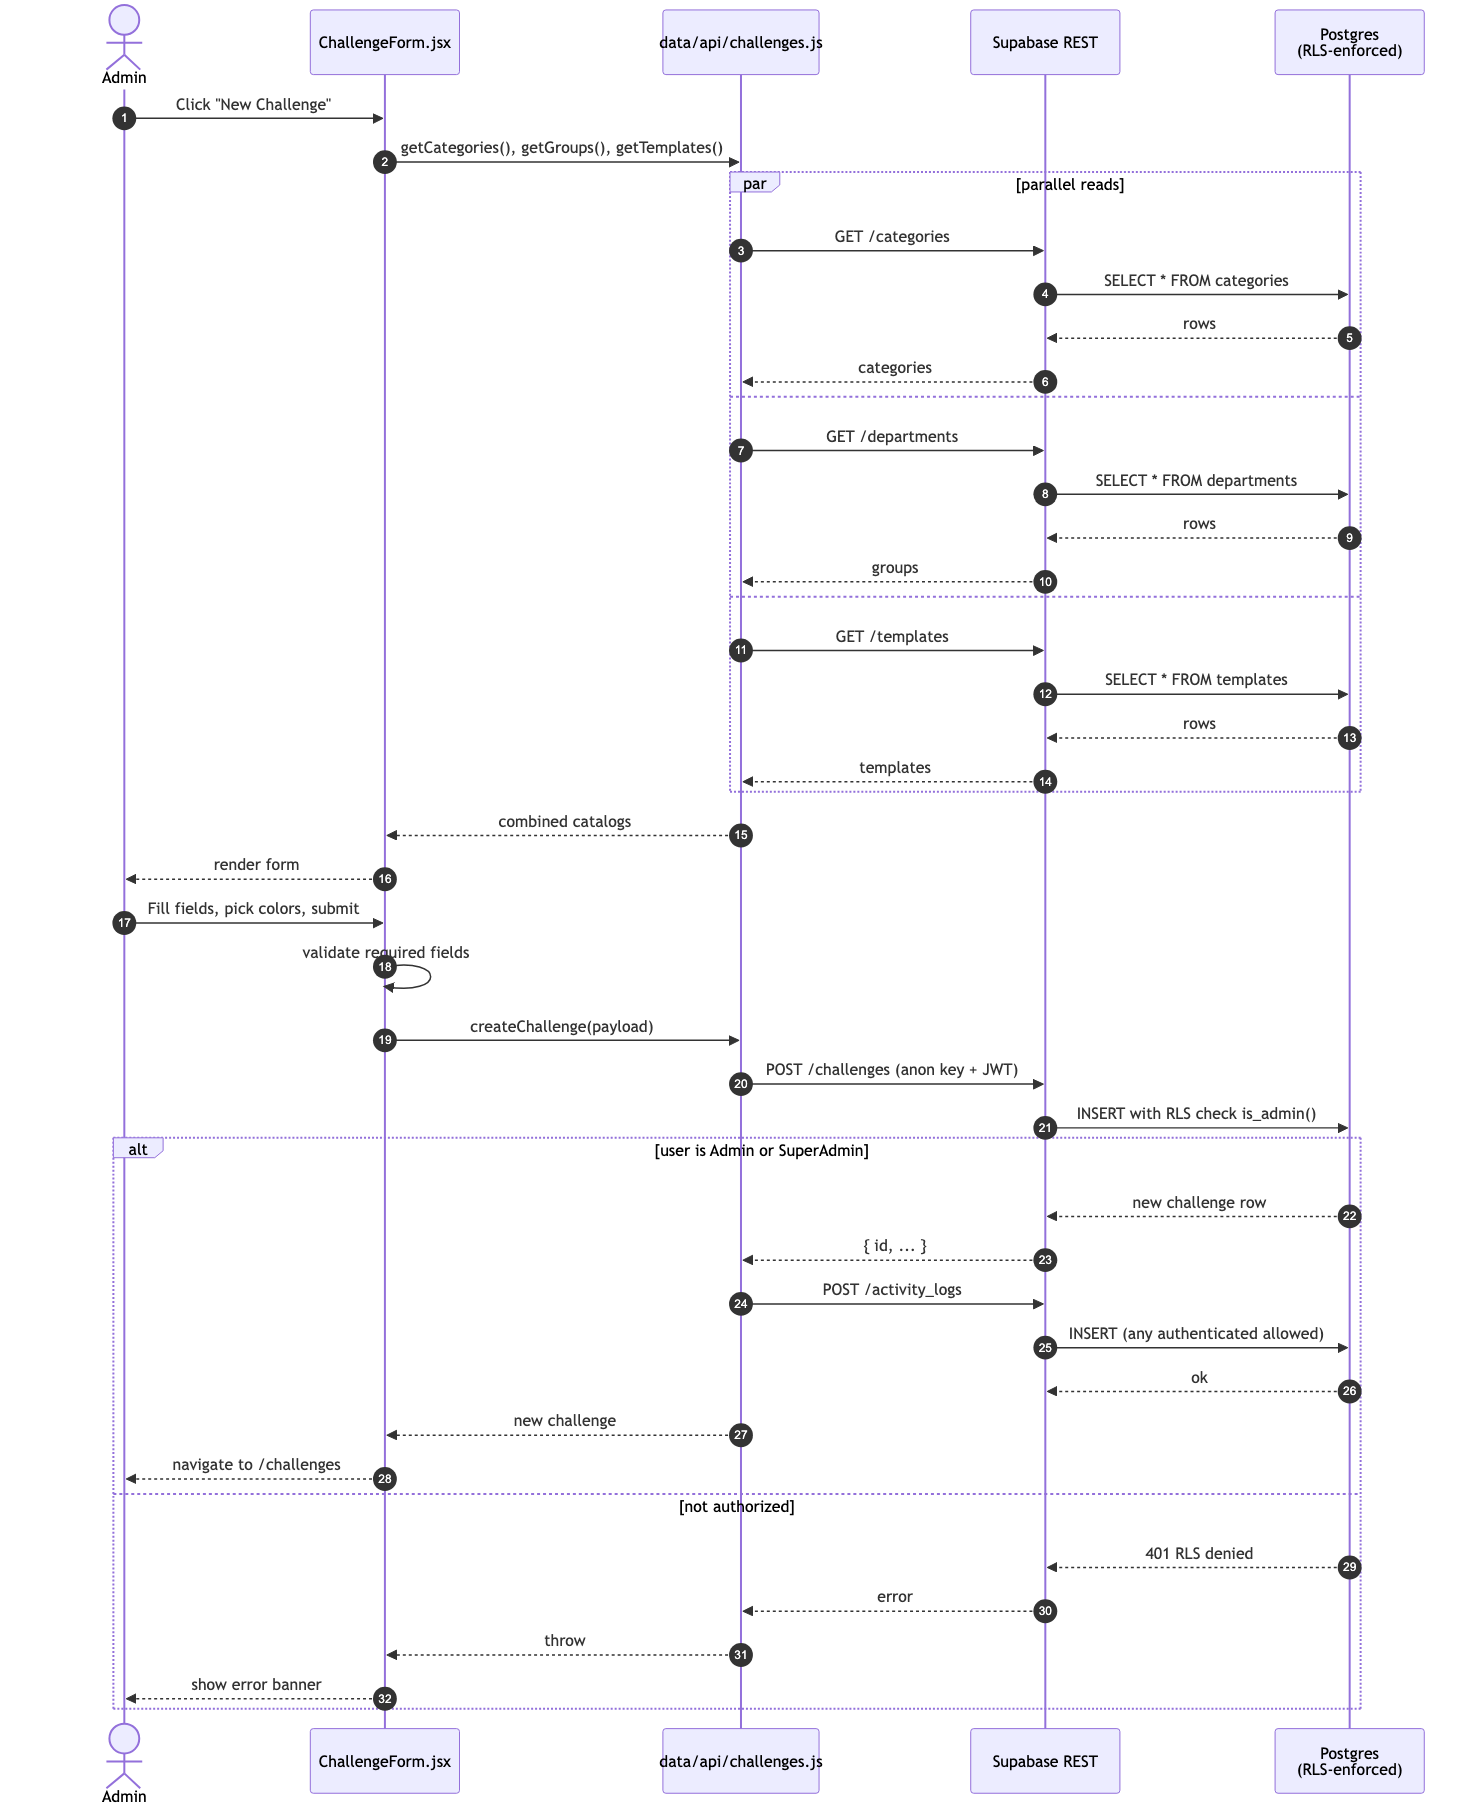
\includegraphics[width=\linewidth]{diagrams/06_seq_create_challenge.png}
  \caption{Sequence diagram -- creating a new challenge. The
  \texttt{admin\_write} RLS policy on the \texttt{challenges}
  table denies the INSERT for callers whose JWT role is not
  Admin or SuperAdmin.}
  \label{fig:seq-cc}
\end{figure}

\subsection{Class / Module Design (Data Layer)}

Figure~\ref{fig:class} shows the structure of the
\texttt{data/api} module. The \texttt{index.js} barrel is the
sole public surface; components are forbidden by ESLint rule
from reaching into sub-modules.

\begin{figure}[H]
  \centering
  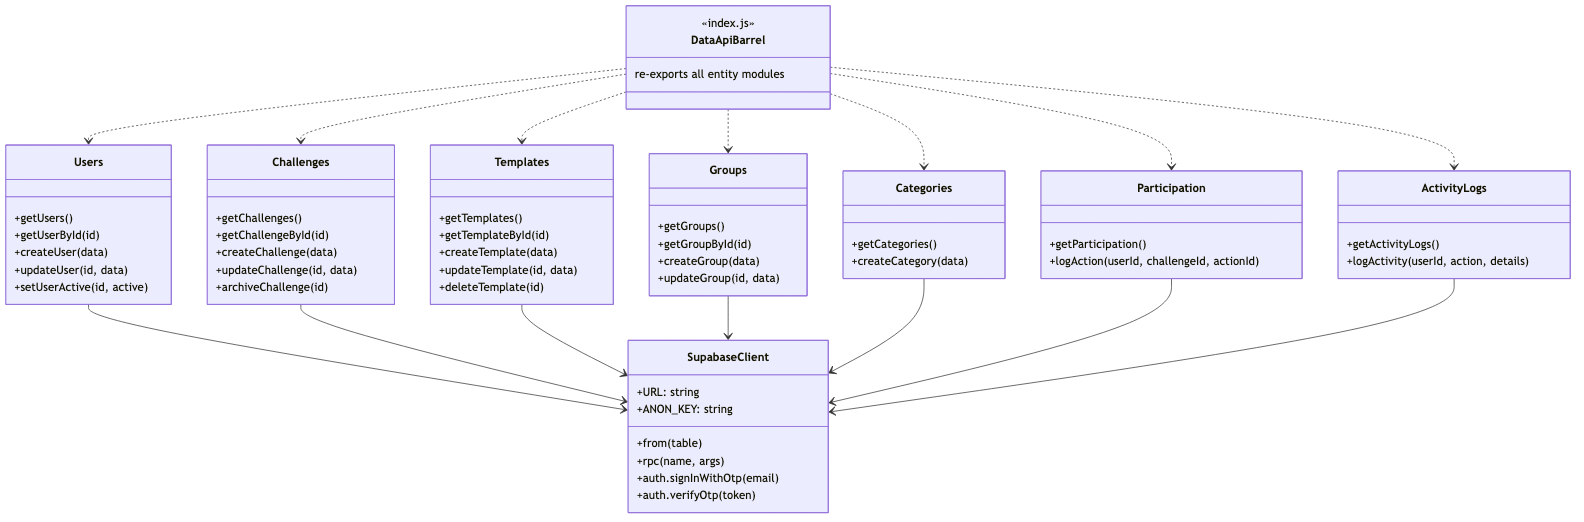
\includegraphics[width=0.95\linewidth]{diagrams/10_class_data_layer.png}
  \caption{Data-layer module structure. Each per-entity module
  owns one Postgres table's CRUD operations.}
  \label{fig:class}
\end{figure}

\subsection{Algorithm Explanation: Auto-Create Theme on Challenge Submit}

When an admin clicks \textbf{Create Challenge}, the form must
reconcile its UI -- which exposes free-form color pickers --
with the schema, which stores colors inline on \texttt{challenges}.
The algorithm in pseudocode:

\begin{lstlisting}[language=Python,caption={Algorithm: build challenge payload for INSERT},captionpos=b]
def build_challenge_payload(form, global_categories, user):
    # 1. Resolve the chosen category name to its FK id.
    category = find(global_categories, name == form.category)
    if not category:
        raise UserVisibleError("Please select a category.")

    # 2. Compose the challenge row, including the four split
    #    color columns.
    return {
        "name":          form.name,
        "description":   form.description,
        "categoryId":    category.id,
        "groupId":       form.groupId or None,
        "startDate":     form.startDate,
        "endDate":       form.endDate,
        "status":        form.status,
        "bgColorHeader": form.bgColorHeader,
        "txColorHeader": form.txColorHeader,
        "bgColorBody":   form.bgColorBody,
        "txColorBody":   form.txColorBody,
        "createdBy":     user.id,
    }
\end{lstlisting}

\subsection{Deployment Plan}

Figure~\ref{fig:deploy} shows the production deployment topology.

\begin{figure}[H]
  \centering
  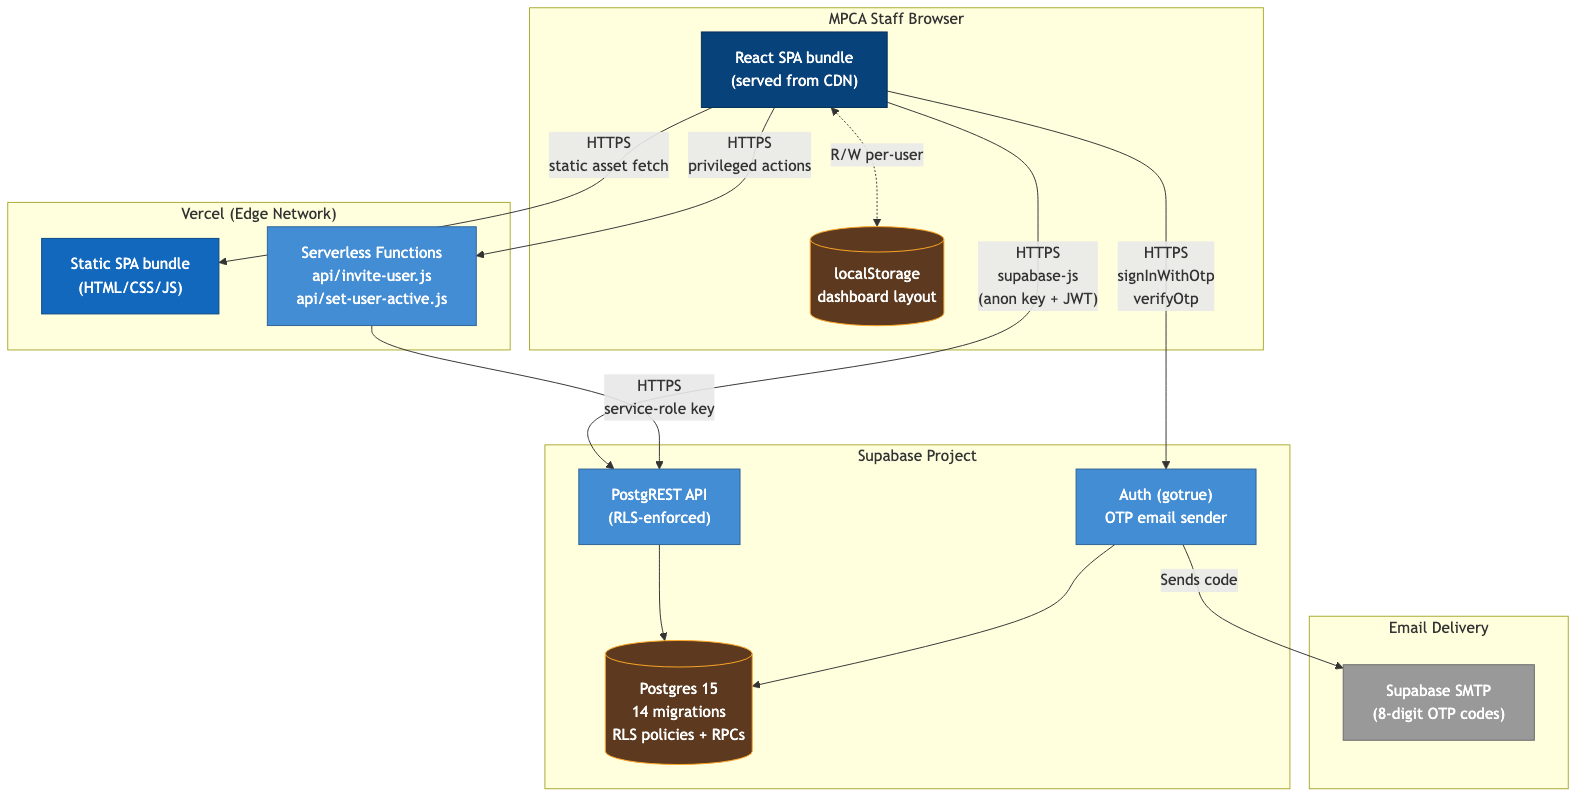
\includegraphics[width=\linewidth]{diagrams/07_deployment.png}
  \caption{Deployment diagram. The SPA is served from Vercel's
  edge network; data and auth go directly to Supabase. Two
  serverless functions handle privileged operations using
  Supabase's service-role key.}
  \label{fig:deploy}
\end{figure}

\subsubsection*{Continuous deployment}

\begin{itemize}[noitemsep]
  \item Push to \texttt{main} triggers a Vercel production
        deploy. Pull requests trigger preview deploys with their
        own URL.
  \item Database changes are version-controlled in
        \texttt{supabase/migrations/} and applied via
        \texttt{supabase db push}. The CLI reconciles the local
        file list against the
        \texttt{supabase\_migrations.schema\_migrations} table on
        the live database.
  \item Environment variables (\texttt{VITE\_SUPABASE\_URL},
        \texttt{VITE\_SUPABASE\_ANON\_KEY}) are set in the Vercel
        project; the service-role key lives only in the
        serverless-function environment and never reaches the
        client bundle.
\end{itemize}

\newpage

% =====================================================================
\section{Source Code Documentation}
% =====================================================================

\subsection{Code Structure}

The application source lives under \texttt{src/admin-app/src/} and
is organized by feature, not by file type. Every page is a feature
folder; cross-cutting components live in \texttt{components/shared/};
all data access goes through \texttt{data/api/}.

\begin{lstlisting}[caption={Source tree (abbreviated)},captionpos=b]
src/admin-app/src/
+- main.jsx                       React entry
+- App.jsx                        Route table
+- lib/
|  +- theme.js                    MUI dark theme
|  +- permissions.js              can(role, perm)
|  +- constants.js                Palettes, status maps
+- components/
|  +- layout/                     AdminLayout, Sidebar, TopBar
|  +- shared/
|     +- feedback/                ConfirmDialog
|     +- data/                    StatCard, CSVExport, EntityLink
|     +- forms/                   ActionFormDialog, CategoryFormDialog
|     +- preview/                 MobilePreview
+- data/
|  +- supabase.js                 sole importer of @supabase/supabase-js
|  +- api/
|     +- index.js                 barrel; the only file features import
|     +- users.js, challenges.js, templates.js, groups.js, ...
+- features/
   +- auth/                       LoginPage, AuthContext, RequireAuth
   +- dashboard/                  22 widgets, ComparisonMode
   +- challenges/                 List, Form, Detail, +10 sub-components
   +- templates/                  List, Form, +1 sub
   +- groups/                     List, Form, Detail, +2 sub
   +- users/                      List, Form, Detail, +5 sub
   +- reports/                    ReportsPage
\end{lstlisting}

\subsection{Naming Conventions}

\begin{itemize}[noitemsep]
  \item \textbf{Files.} React components use \texttt{PascalCase.jsx}
        (e.g.\ \texttt{ChallengeForm.jsx}). Hooks use
        \texttt{useCamelCase.js}. Non-component modules use
        \texttt{camelCase.js} (e.g.\ \texttt{aggregations.js}).
  \item \textbf{Folders.} Feature folders are plural nouns
        (\texttt{challenges/}, \texttt{users/}). Component sub-folders
        are singular nouns (\texttt{components/shared/feedback/}).
  \item \textbf{Variables and functions.} \texttt{camelCase}.
        React event handlers prefixed with \texttt{handle}
        (\texttt{handleSubmit}, \texttt{handleApplyTemplate}).
        Props that are callbacks prefixed with \texttt{on}
        (\texttt{onChange}, \texttt{onSelect}).
  \item \textbf{Constants.} \texttt{UPPER\_SNAKE\_CASE}
        (\texttt{CHALLENGE\_STATUSES}, \texttt{ROLES}).
  \item \textbf{Database columns.} Postgres identifiers use
        \texttt{camelCase} (quoted, e.g.\ \texttt{"groupId"}). Table
        names are plural \texttt{snake\_case}
        (\texttt{challenge\_participants}). Foreign keys end in
        \texttt{Id} (\texttt{userId}, \texttt{challengeId}).
\end{itemize}

\subsection{Commenting Standards}

\subsubsection*{File-header docblock}

Every source file opens with a JSDoc block giving a one-line
\texttt{@summary} and any context the file's purpose can't convey
on its own:

\begin{lstlisting}[language=Java,caption={Example file-header docblock},captionpos=b]
/**
 * @file ChallengeForm.jsx
 * @summary ChallengeForm -- create or edit a challenge.
 *
 * Renders three sub-views, all under one route:
 *   - TemplatePicker: only on create, lets the user pre-fill from a template
 *   - ChallengeFieldsSection: the field grid
 *   - ActionsEditor: only on edit, manages the challenge's actions
 *
 * This component owns the form state and the submit pipeline; the
 * sub-components are pure presentational.
 */
\end{lstlisting}

\subsubsection*{JSDoc on exported functions}

Every exported function carries a JSDoc block declaring its
parameters and return shape. Generated documentation is not
shipped; the value is in-IDE hover and onboarding.

\subsubsection*{Inline comments explain \emph{why}, not \emph{what}}

Inline comments justify non-obvious decisions; they never
restate what the code already says.

\begin{lstlisting}[language=Java,caption={Example: a \emph{why} comment},captionpos=b]
// security definer + explicit search_path so the inner SELECT
// bypasses RLS on public.users (otherwise the admin_write policy
// would recursively call this function while evaluating itself).
create or replace function public.current_user_role() ...
\end{lstlisting}

\subsubsection*{TODO and FIXME format}

\texttt{TODO(name): short description -- issue\#NN} or
\texttt{FIXME(name): ...}. Every TODO points to a tracked
GitHub issue so the next developer can find the context.

\subsection{Style Enforcement}

\begin{itemize}[noitemsep]
  \item \textbf{Prettier} owns whitespace, quote style, semicolons,
        and line length. Configured via \texttt{.prettierrc.json};
        runs in CI and on \texttt{npm run format}.
  \item \textbf{ESLint flat config} enforces import order, no-unused,
        max-lines, and the React recommended set. Custom rule:
        no file in \texttt{src/admin-app/src/} may exceed 300 lines
        of code; offenders fail the lint job.
  \item \textbf{File-size policy.} Components over 200 lines are
        candidates for decomposition; over 300 lines is a hard cap.
        See the version-history entries for v0.7.0 and v0.7.1 for
        the project-wide decomposition that brought every file
        under the cap.
\end{itemize}

\newpage

% =====================================================================
\section{QA Activities Document}
% =====================================================================

\subsection{Test Strategy}

The team adopted a pragmatic, manual-first test strategy
appropriate to a one-semester capstone:

\begin{itemize}[noitemsep]
  \item \textbf{Static analysis} on every commit: ESLint catches
        unused imports, React Hooks rule violations, and the
        300-line cap; Prettier catches formatting drift.
  \item \textbf{Build verification} on every pull request: Vercel
        builds a preview deploy from the PR's HEAD. A red build is
        a blocking merge condition.
  \item \textbf{Manual exploratory testing} on the preview URL
        before merging each PR. Each PR description carries an
        explicit ``Test plan'' checklist (see for example PRs
        \#81, \#83, \#85).
  \item \textbf{Schema reconciliation} on every migration:
        \texttt{supabase db push --dry-run} is run against the
        live project to confirm only intended migrations would be
        applied; \texttt{supabase migration list --linked} is
        diffed against the local file list to confirm no drift.
\end{itemize}

\subsection{Test Cases}

The table below documents the exploratory-test pass that
verified each user story and major use case for the final
release. \textit{Expected} is the acceptance criterion;
\textit{Actual} is the observed behavior on the production
deploy.

\begin{longtable}{p{0.06\linewidth} p{0.27\linewidth} p{0.31\linewidth} p{0.27\linewidth} p{0.05\linewidth}}
\toprule
\textbf{ID} & \textbf{Scenario} & \textbf{Expected} & \textbf{Actual} & \textbf{P/F} \\
\midrule
TC-1 & Login: unregistered email & ``Email not recognized'' shown; no code sent. & Matches expected. & P \\
TC-2 & Login: deactivated user & ``Account deactivated'' shown; no code sent. & Matches expected. & P \\
TC-3 & Login: valid email, correct code & User is signed in and lands on dashboard within 2s. & Matches expected. & P \\
TC-4 & Login: valid email, wrong code & Inline error; form remains populated. & Matches expected. & P \\
TC-5 & Create group (Admin) & Group appears immediately in list with 0/0 counts. & Matches expected. & P \\
TC-6 & Create group (GeneralUser) & ``New Group'' button is not rendered. & Button hidden; direct POST attempt is denied by RLS. & P \\
TC-7 & Create challenge from template & Form pre-fills; actions stage; redirect to /challenges after save. & Matches expected. & P \\
TC-8 & Create challenge: missing required field & Browser-native validation blocks submit. & Matches expected. & P \\
TC-9 & Dashboard: drag-and-drop reorder & New position persists across hard refresh. & Matches expected. & P \\
TC-10 & Dashboard: apply preset & Visible layout changes; Save persists; Cancel restores. & Matches expected. & P \\
TC-11 & Reports: filter by challenge + date & Row count updates; CSV exports filtered rows. & Matches expected. & P \\
TC-12 & Reports: empty filter & Empty state shown; Export disabled. & Matches expected. & P \\
TC-13 & User detail: change group (Admin) & Group updates immediately; audit log row written. & Matches expected. & P \\
TC-14 & User detail: deactivate (SuperAdmin) & User flips to Deactivated; cannot log in. & Matches expected. & P \\
TC-15 & Mobile preview updates live & Typing in form fields updates the preview. & Matches expected. & P \\
\bottomrule
\end{longtable}

\subsection{Defect Reports}

The following defects were filed, fixed, and verified during
the spring 2026 release cycle. Severity uses a four-tier scale
(Critical / High / Medium / Low). All listed defects are
closed.

\subsubsection*{DR-1 -- Create Challenge button silently fails (\#82)}

\begin{itemize}[noitemsep]
  \item \textbf{Severity:} Critical -- core user story (US-2,
        UC-1) blocked.
  \item \textbf{Reproduce:} On the live deploy, click
        \textbf{New Challenge}, fill all required fields, click
        \textbf{Create Challenge}.
  \item \textbf{Expected:} Challenge is created; redirect to
        \texttt{/challenges}.
  \item \textbf{Actual:} Browser console showed
        \texttt{POST /rest/v1/challenges?select=* 400 (Bad
        Request)} with PostgREST error ``Could not find the
        'bgColorBody' column of 'challenges' in the schema
        cache''; no user-visible feedback.
  \item \textbf{Root cause:} The form had always written the
        four split-color columns
        (\texttt{bgColorHeader}/\texttt{txColorHeader}/\texttt{bgColorBody}/\texttt{txColorBody}),
        but the deployed schema only carried the legacy single
        \texttt{theme text} column. The repository's
        \texttt{001\_initial\_schema.sql} described a different
        normalized schema that was never deployed, misleading
        the initial fix attempt.
  \item \textbf{Fix:} Added migration
        \texttt{014\_challenge\_split\_colors.sql} adding the
        four columns, applied via \texttt{supabase db push}.
        Merged in PR~\#83. Subsequently issued PR~\#85 to
        reconcile the in-repo migration files with the
        actually-deployed schema and squash 14 migrations to
        2 for handoff readability.
  \item \textbf{Status:} Closed; verified on production by
        creating a challenge end-to-end.
\end{itemize}

\subsubsection*{DR-2 -- Dev login race condition}

\begin{itemize}[noitemsep]
  \item \textbf{Severity:} High -- blocked dev productivity for
        the whole team after the RLS migration.
  \item \textbf{Reproduce:} Click ``Quick Login as Kristin'';
        observe that the dashboard renders before
        \texttt{user.role} is populated, causing role-gated
        widgets to flicker.
  \item \textbf{Expected:} Dashboard does not render until the
        app user row is loaded.
  \item \textbf{Actual:} Caller's \texttt{navigate("/")} fired
        before \texttt{RequireAuth} could see the new user.
  \item \textbf{Fix:} Load the app user inline inside
        \texttt{devLogin} before returning success. Merged as
        commit \texttt{ef9f3c5}.
  \item \textbf{Status:} Closed; verified by repeated Quick
        Login attempts with no flicker.
\end{itemize}

\subsubsection*{DR-3 -- Magic-link tokens consumed by corporate email scanners}

\begin{itemize}[noitemsep]
  \item \textbf{Severity:} High -- blocked real users at MPCA
        even though local dev was unaffected.
  \item \textbf{Reproduce:} Send a magic-link to an
        \texttt{@mpca.mn.gov} account; click the link in the
        email.
  \item \textbf{Expected:} Successful sign-in.
  \item \textbf{Actual:} Sign-in fails with ``token already
        consumed.'' Microsoft Defender Safe Links pre-fetches
        the URL on email arrival, burning the one-time token
        before the user can click it.
  \item \textbf{Fix:} Migrated the auth flow from magic links
        to an 8-digit OTP code in PR~\#61. Code is delivered
        in plain text in the email body, which scanners do not
        pre-fetch.
  \item \textbf{Status:} Closed; verified on a live MPCA email
        account.
\end{itemize}

\subsubsection*{DR-4 -- Cross-feature component imports}

\begin{itemize}[noitemsep]
  \item \textbf{Severity:} Low -- code-quality issue, no
        user-visible effect.
  \item \textbf{Reproduce:} \texttt{grep -r "features/challenges" src/admin-app/src/features/}.
  \item \textbf{Expected:} No feature folder imports another
        feature's components.
  \item \textbf{Actual:} \texttt{features/templates/TemplateForm.jsx}
        imported \texttt{ActionFormDialog} and
        \texttt{CategoryFormDialog} from
        \texttt{features/challenges/components/}.
  \item \textbf{Fix:} Moved both dialogs into
        \texttt{components/shared/forms/} and updated import
        sites. Merged as PR~\#81 (closes \#70).
  \item \textbf{Status:} Closed; the architectural invariant
        is now enforced by convention and verified by grep.
\end{itemize}

\subsection{Known Limitations}

The following are documented limitations rather than defects;
they are out of scope for the spring 2026 capstone and are
flagged for the next student team.

\begin{itemize}[noitemsep]
  \item No integration with the Team 1 mobile app beyond
        sharing the database schema.
  \item Dashboard layout persists to \texttt{localStorage}
        only; not synced across devices.
  \item \texttt{presets} and \texttt{preset\_actions} legacy
        tables still exist on the live database even though
        the application no longer reads them; safe to drop in
        a future migration.
  \item The legacy \texttt{challenges.theme} single-color
        column is still read by some dashboard widgets while
        the form writes only the four split-color columns;
        widget code should migrate to read the split columns
        in a follow-up.
\end{itemize}

\newpage

% =====================================================================
\section*{References}
\addcontentsline{toc}{section}{References}
% =====================================================================

\begin{enumerate}[label={[\arabic*]}]
  \item S. Brown, \emph{The C4 model for visualising software
        architecture}. [Online]. Available:
        \url{https://c4model.com/}. [Accessed: May 21, 2026].
  \item Supabase, ``Row Level Security.'' [Online]. Available:
        \url{https://supabase.com/docs/guides/auth/row-level-security}.
        [Accessed: May 21, 2026].
  \item Supabase, ``Database Migrations.'' [Online]. Available:
        \url{https://supabase.com/docs/guides/deployment/database-migrations}.
        [Accessed: May 21, 2026].
  \item Material UI, ``Material UI v7 Documentation.'' [Online].
        Available: \url{https://mui.com/material-ui/}. [Accessed:
        May 21, 2026].
  \item Vercel, ``Functions Overview.'' [Online]. Available:
        \url{https://vercel.com/docs/functions}. [Accessed: May
        21, 2026].
  \item J. Patton, \emph{User Story Mapping: Discover the Whole
        Story, Build the Right Product}. O'Reilly Media, 2014.
  \item W3C, ``Web Content Accessibility Guidelines (WCAG) 2.1.''
        [Online]. Available: \url{https://www.w3.org/TR/WCAG21/}.
        [Accessed: May 21, 2026].
  \item Mermaid, ``Mermaid Documentation.'' [Online]. Available:
        \url{https://mermaid.js.org/}. [Accessed: May 21, 2026].
\end{enumerate}

\end{document}
